\section{Problem 4}

{\bfseries 4.1 Part1}

\begin{figure}[!htb]
\minipage{0.25\textwidth}
  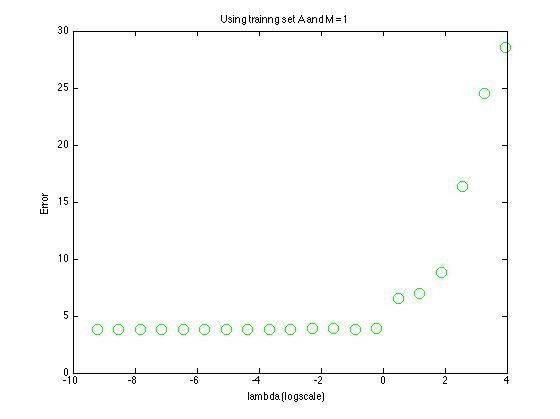
\includegraphics[width=\linewidth]{figures/p4_LAD_regressA_m=1}
\endminipage\hfill
\minipage{0.25\textwidth}
  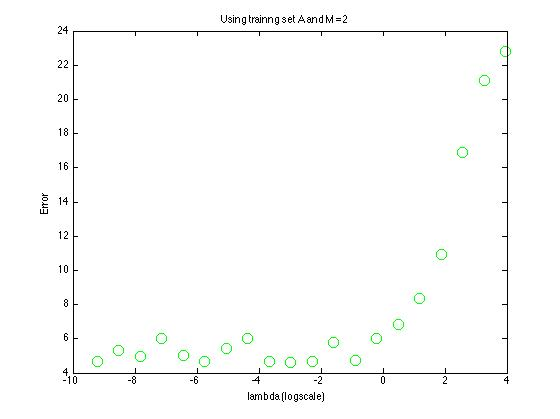
\includegraphics[width=\linewidth]{figures/p4_LAD_regressA_m=2}
\endminipage\hfill
\minipage{0.25\textwidth}                                                                                 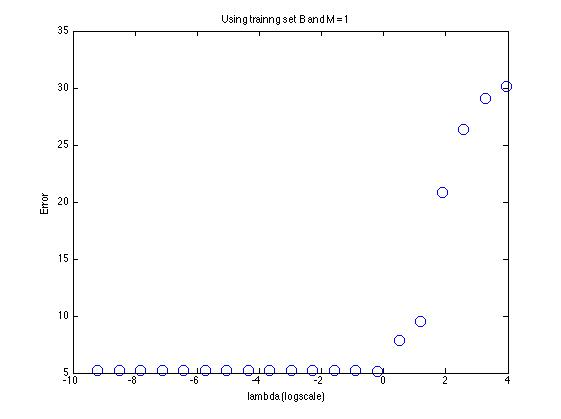
\includegraphics[width=\linewidth]{figures/p4_LAD_regressB_m=1}
\endminipage\hfill
\minipage{0.25\textwidth}
  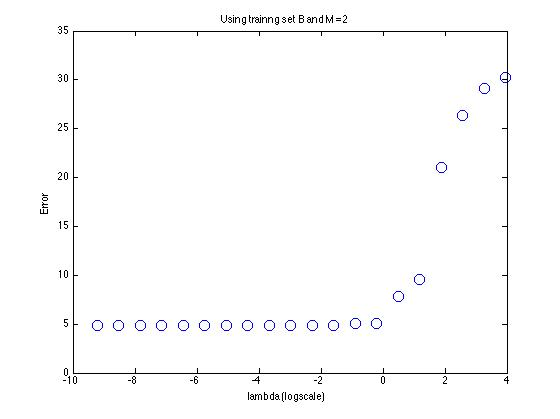
\includegraphics[width=\linewidth]{figures/p4_LAD_regressB_m=2}
\endminipage\hfill
\caption{LAD for set A,B and M = 1,2}\label{p4_LAD}
\end{figure}

Again we splitted the validation set into a validation and test set. Figure~\ref{p4_LAD} shows the result for M = 1,2 for LAD (green is trained using A, blue is trained with B). My experiments on validation set shows that M = 1, M = 2 generates the best results using both A and B. We carried out a series of experiments with varying values of lambda, setting M = 2 and 3. The lambdas on x axis is in log scale. The error for LAD is measured using the absolute value loss function because the model is optimized for this loss function. I tested a few configurations with M = 3 and M = 4, but the error is larger than that of the best M = 2 configurations. We then evaluated the best M,lambda pair on the test set. We verified the correctness of the algorithm by plotting a few configurations on the training and validation data. 

We first notice that the model generated from training set B's error
is comparable to the models generated from training set A. The minimum of
both models is around 5. The low error for B is because that the 
LAD model uses an absolute value based loss function that penalizes less
on outliers compare to the squared error loss function. Additionally, as the error is small for both models. There is no clear minimum point as we increase the lambda (or it is very samll). We chose the best M and lambda for A (M = 2, lambda = 0.01) , for B (M = 2, lambda = 0.01) using the LAD's loss function.  Then, we tested the two models on the test set. The error we see on the test set is very similar to the error in the validation set. 


{\bfseries 4.2 Part2}
\begin{figure}[!htb]
\minipage{0.25\textwidth}
  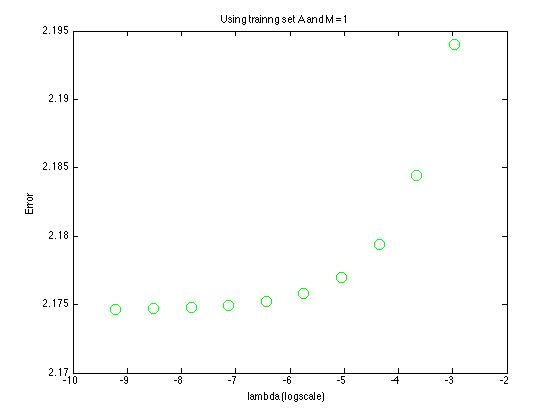
\includegraphics[width=\linewidth]{figures/p4_LASSO_regressA_m=1}
\endminipage\hfill
\minipage{0.25\textwidth}
  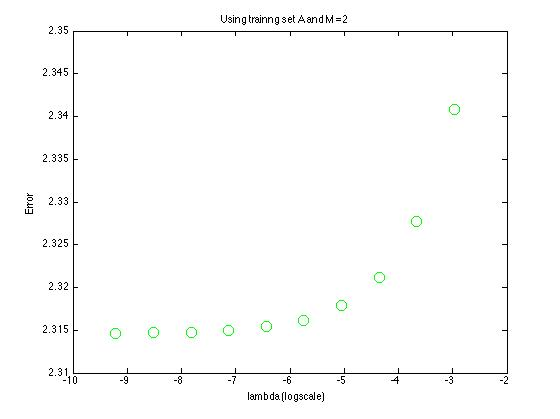
\includegraphics[width=\linewidth]{figures/p4_LASSO_regressA_m=2}
\endminipage\hfill
\minipage{0.25\textwidth}                                                                                 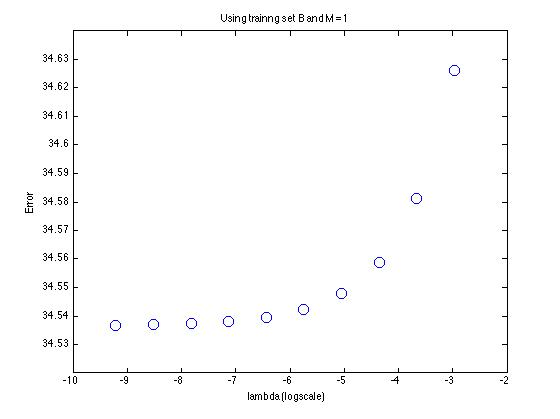
\includegraphics[width=\linewidth]{figures/p4_LASSO_regressB_m=1}
\endminipage\hfill
\minipage{0.25\textwidth}
  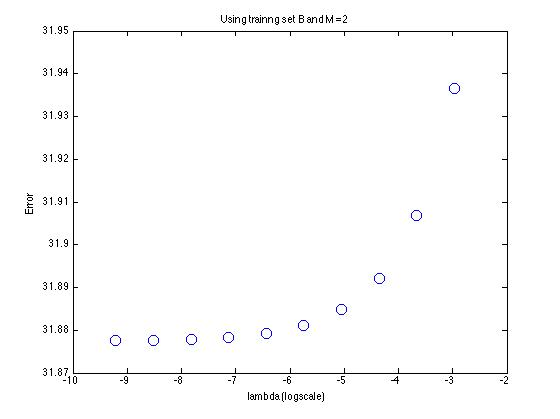
\includegraphics[width=\linewidth]{figures/p4_LASSO_regressB_m=2}
\endminipage\hfill
\caption{LASSO validation error using set A, M = 1,2 and B, M = 1,2}\label{fig:p4_LASSO}
\end{figure}

The configuration for the tests are similar to that described in part 1. The results are shown in figure~\ref{fig:p4_LASSO}. We used LASSO for generating models and squared errors for selecting model using validation data. Again we generated a few data point for M = 3 and M = 4, but we noticed that the validation error is high for the data points. For M = 4, some data points become hard to converge. We have to choose a very samll size.  
 
We first notice that training set B has much higher error rate than using training set A when lambda is less than 0.01. This is because LASSO still uses a L2 norm as its loss function. As a result, the tolerance for the outlier in data set B is low. Second,we can see the error rate for LASSO increases quickly for M = 2 and M = 3 using both A and B as training data. Lastly, we found that some of the elements in the weight vector for M =3, 4 are driven close to 0 because the L1 norm regularization drives some weight to 0 easily (the weights are more sparse).  

{\bfseries 4.3 Part3}

We want to use the least absolute deviations when there are outliers in your training data. Compare the last two figures in figure~\ref{fig:p4_LAD} and~\ref{p4_LASSO}, model trained using LAD has lower error and better tolearance for outlier compared to LASSO and SSE on training set B. When we are confident about the quality of the data (very few or no outliers), then using a squared error loss function would be more accurate in training the model. LASSO uses L1 norm for regularization to make the weight factors more sparse. 

